\section{Windows}
\subsection{Historique}
Descendant de MS-DOS (\textit{Microsoft Disk Operating System}) créé en 1981
par Bill Gates, Paul Allen et Steve Ballmer. Ce n'est que le 20 novembre 1985
que la première version de Windows apparut (\textit{Windows 1.0}) offrant la
possibilité d'utiliser une interface graphique sans devoir taper des commandes
MS-DOS. \\

20 jours plus tard, Windows 2.0 voit le jour offrant la possibilité de faire se
chevaucher des fenêtres, de contrôler la disposition de l'écran ainsi que de
faire l'usage de raccourcis clavier. En 1988, les ordinateurs commencent à
faire partie du quotidien de divers employés de bureau. \\

Windows 3.0 fut annoncé le 22 mai 1990 et la version 3.1 sera disponible en
1992. Suite à cela, Windows dispose désormais de meilleures performances d'un
point de vue graphismes puisqu'il peut supporter 16 couleurs et possède une
amélioration concernant les icônes. \\

Remarque : Windows NT, sorti le 27 juillet 1993, sera intéressant d'un point de
vue commercial puisque celui-ci est un système d'exploitation 32 bits. \\

Dans la suite de l'évolution, Windows 95 sort le 24 août 1995 offrant les
fonctionnalités de base que nous connaissons aujourd'hui tel que le bouton
Démarrer, l'heure des fax/modems, du courrier électronique, de l'univers en
ligne et des jeux multimédias et logiciels éducatifs, ... \\

À ce moment, 80 \% des PC du monde entier utilisent Windows et MS-DOS. \\

Le 25 juin 1998, Windows 98 est rendu disponible et devient la première
version de Windows spécialement conçue pour les utilisateurs. Les PC sont dès à
présent disponibles tout autour de nous, que ce soit dans les bureaux, à la
maison ou dans des cybercafés. Cette version sera la dernière version basée sur
MS-DOS. \\

Toujours dans l'utilisation domestique, Windows Me proposera des \\
perfectionnements pour la musique, la vidéo et le réseau domestique, ... \\

Dès lors, Microsoft annonce que tous les prochains systèmes d'exploitation
seront basés sur le noyau de Windows NT et de Windows 2000. \\

Windows 2000 Professionnel simplifie entre autres l'installation matérielle en
considérant la prise en charge de matériels Plug-and-Play, comprenant des
produits sans fil et réseau, des périphériques USB, des périphériques IEEE-1394
et des périphériques infrarouges. \\

L'un des produits les plus vendus au cours des prochaines années sera Windows
XP disponible à partir du 25 octobre 2001 et qui sera proposé en plusieurs
versions (64 bits, Media Center, Tablet PC). Effectivement, celui-ci sera
fourni dans 25 langues et offrant une nouvelle ergonomie ciblée sur
l'utilisation et le centre unifié de services d'aide et d'assistance. \\

En 2006, Windows Vista est annoncé visant à renforcer la sécurité à l'aide d'un
contrôle de compte d'utilisateur, en apportant un lecteur de chiffrement
BitLocker, ... \\

Néanmoins, cette version de Windows fut beaucoup critiquée suite aux nombreux
logiciels provenant de Windows XP incompatibles avec cette version. \\

En 2009, Microsoft introduit l'interface tactile à l'aide de Windows 7 vu qu'il
est devenu courant de se connecter dans des zones d'accès sans fil. \\

Suivant cette direction, Windows 8 - conçu en 2012 - propose une toute nouvelle
interface compatible à la fois avec un clavier et une souris ainsi qu'avec la
technologie tactile. \\

Puis, après la version Windows 8.1, Windows 10 est enfin arrivé et est, d'après
Microsoft, le meilleur Windows jamais créé. Cette version dispose d'une
assistante personnelle intelligente (\textit{Cortana}). \\

\begin{figure}[!htb] \minipage{0.45\textwidth}
  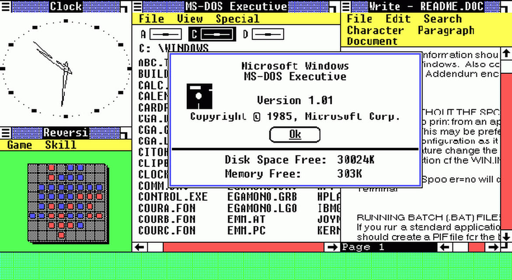
\includegraphics[width=\linewidth]{textures/images/windows/historic/Win1.png}
  \caption{Windows 1.01}\label{fig:Windows 1.01}
	\endminipage\hfill \minipage{0.45\textwidth}
  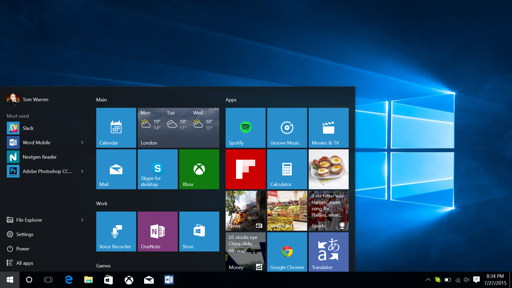
\includegraphics[width=\linewidth]{textures/images/windows/historic/Win10.png}
  \caption{Windows 10}\label{fig:Windows 10}
	\endminipage
\end{figure}

\clearpage

\subsection{Utilisation}
Windows étant le premier système d'exploitation pour les PC en terme de part de
marché, il est aisé de savoir le pourquoi du comment de cette position. \\

Premièrement, il faut savoir que Windows est le système d'exploitation installé
par défaut sur tous les ordinateurs. De ce fait, lors de l'achat de
l'ordinateur, Windows est fourni avec celui-ci. \\

Remarque : il est possible d'acheter un ordinateur directement avec GNU/Linux
sur des sites commerciaux en technologie tels que \textit{LDLC} et
\textit{system76}, ce qui permet de réduire le prix initial de l'ordinateur. \\

De plus, la plupart des développeurs s'occupent en priorité de la compatibilité
sur Windows permettant de rendre leurs logiciels accessibles pour un public
beaucoup plus vaste. \\

Windows a également l'avantage de regrouper diverses catégories de personne. On
y retrouve des adolescents dont leur demande première se trouve dans
l'utilisation de jeux vidéo, des adultes voulant profiter des fonctionnalités
standards qu'offre un système d'exploitation, des personnes âgées, ... \\

Autrement dit, Windows est un système d'exploitation universel regroupant une
large communauté de personnes ce qui offre l'avantage de trouver une réponse
très facilement face à un problème ou une question spécifique sur l'OS. \\

Il est également possible d'utiliser cet OS sur son téléphone.
Effectivement, des smartphones sont équipés de Windows Phone. Même si celui-ci
est moins répandu qu'Android et iOS, il a l'avantage d'être très rapide sur de
petites configurations et d'offrir des téléphones à prix raisonnable. La
principale raison à cela est que de nombreuses applications ne fonctionnent que
pour Android ou iOS. \\

Néanmoins, certains spécialistes en la matière considèrent que Windows Phone
n'est pas rentable pour Microsoft et qu'il ne sera plus mis à jour dans le
futur. De ce fait, les utilisateurs de Windows Phone devront opter pour Android
ou iOS si ça devait être le cas.

\clearpage

\subsection{Mobile}

Tout comme Apple, Nokia et Samsung, Microsoft possède une longue histoire dans
le mobile. Entre les PDA, les tablettes et les téléphones, ces firmes ont
développé des systèmes d'exploitation mobiles spécialement conçus pour ces
appareils. \\

La première version de ce système est nommée \textit{Pocket PC 200} et est basée
sur une version de Windows spécialement prévue pour des appareils possédant
peu de ressources - Windows CE. \\

Au fil des ans, le nom devient Windows Mobile 2003 puis Windows Mobile 5. Sur
cette version, on peut retrouver une adaptation de Microsoft Office. \\

Avec la sortie de l'iPhone en 2007 suivi très rapidement par Samsung (avec Android),
Windows Mobile est à la traîne. C'est pourquoi Microsoft présente Windows Phone 7
au public en 2011. Pendant ce temps, Windows Mobile 6 a connu de grands changements
afin de rester dans la course…

  \begin{figure}[!h]
    \center
    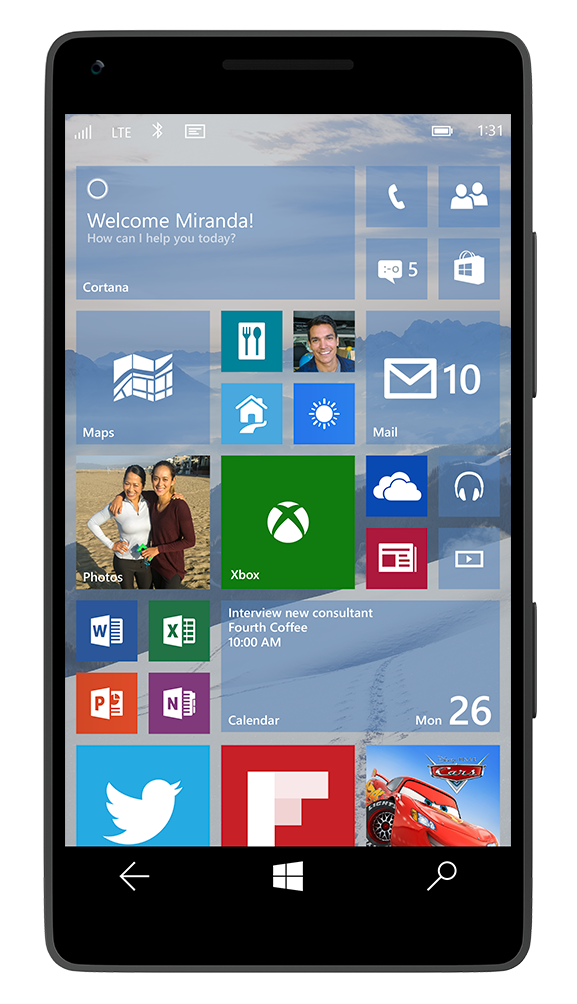
\includegraphics[scale=0.5]
    {textures/images/windows/Windows10Mobile.png}
    \caption{Windows 10 Mobile}
  \end{figure}

La dernière version en date est Windows Mobile 10 qui est très proche de la
version bureau, la politique de Microsoft étant d'avoir un seul et unique
système d'exploitation pour tous les appareils.

\newpage

\subsection{Fonctionnalités}
Le système d'exploitation de la firme de Redmond possède plusieurs fonctionnalités bien à lui. \\

Depuis Windows 10, les applications disponibles dans le Windows Store sont
universelles. Elles peuvent donc tourner sur n'importe quel ordinateur ou
smartphone possédant Windows 10, ainsi que sur les Xbox One et les \textit{HoloLens} ! \\
La suite Microsoft Office est d'ores et déjà universelle. \\

Une autre nouveauté se nomme \textit{Continuum} et consiste à « transformer » sa tablette tantôt en
ordinateur portable, tantôt en tablette. \\
L'utilisateur peut utiliser sa tablette en tant que PC, avec son clavier et une souris,
avec la version PC de Windows 10; puis l'utiliser en \textit{mode tablette}:
le menu Démarrer prend tout l'écran comme dans Windows 8. \\
Pour les Windows Phones, il existe quelque chose de similaire: si l'on branche son
Windows Phone - \textit{muni de Windows 10 Mobile} - à un clavier, une souris et sa station d'accueil
elle-même branchée à un écran, l'écran susmentionné affiche une interface de bureau. Le système
est encore celui de Windows Mobile mais il affiche un menu Démarrer et un \textit{faux} bureau.
Bien entendu, seules les applications universelles peuvent être utilisées dans ce mode. \\

Pour les joueurs possédant une Xbox One, il est possible d’y jouer depuis son ordinateur sous Windows 10. \\

Côté sécurité, depuis Windows 8, il est possible de se connecter à l’aide d’un code à 4 chiffres
comme sur mobiles ou un code gestuel sur une image.
Avec l’arrivée de Windows 10, \textit{Windows Hello} fait son apparition.
La connexion peut s'effectuer à l’aide d’un capteur biométrique, le critère est
désormais le visage (\textit{à l’aide d’une caméra RealSense 3D}), une empreinte digitale ou l’iris.

\begin{figure}[!htb] \minipage{0.45\textwidth}
  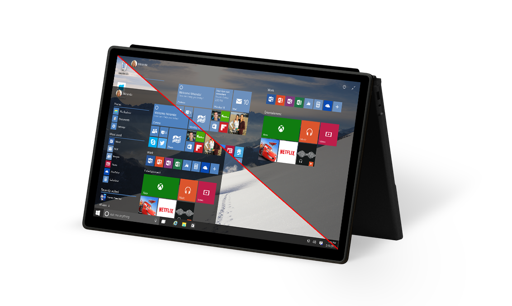
\includegraphics[width=\linewidth]
  {textures/images/windows/features/Continuum_tablet.png}
  \caption{Continuum tablette}\label{fig: Continuum}
	\endminipage\hfill \minipage{0.45\textwidth}
  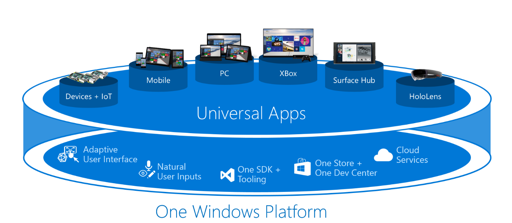
\includegraphics[width=\linewidth]{textures/images/windows/features/Universal_App.png}
  \caption{App universelle}\label{fig:App universelle}
	\endminipage
\end{figure}

\clearpage
